\ifmostrarGabarito
\begin{minted}{python}
import matplotlib.pyplot as plt
from typing import List

def gerar_dashboard_acustico(
    valores_snr: List[float],
    setores: List[str],
    contagens: List[int],
    caminho_img: str
) -> bool:
    """
    Renderiza painel com histograma de SNR e grafico de barras rotulado lado a lado.
    """
    # Cria grade de subgraficos 1 linha x 2 colunas com proporcao panoramica
    fig, (ax1, ax2) = plt.subplots(1, 2, figsize=(13, 5))
    
    # Subgrafico 1: Histograma de distribuicao da relacao sinal-ruido
    ax1.hist(valores_snr, bins=12, color="teal", edgecolor="black", alpha=0.75)
    media_snr = sum(valores_snr) / len(valores_snr) if valores_snr else 0.0
    ax1.axvline(media_snr, color="red", linestyle="--", linewidth=1.8, label=f"Media: {media_snr:.1f} dB")
    ax1.set_title("Distribuicao da Relacao Sinal-Ruido (SNR)", fontsize=11, fontweight="bold")
    ax1.set_xlabel("SNR (dB)", fontsize=10)
    ax1.set_ylabel("Frequencia de Deteccoes", fontsize=10)
    ax1.grid(True, linestyle=":", alpha=0.5)
    ax1.legend(loc="upper right")
    
    # Subgrafico 2: Grafico de barras verticais com contatos por setor
    barras = ax2.bar(setores, contagens, color="steelblue", edgecolor="black", width=0.6)
    # Adiciona rotulos numericos automaticos sobre o topo de cada barra
    ax2.bar_label(barras, padding=3, fontsize=9, fontweight="bold")
    ax2.set_title("Contatos Acusticos por Setor Tatico", fontsize=11, fontweight="bold")
    ax2.set_xlabel("Setor de Varredura", fontsize=10)
    ax2.set_ylabel("Total de Contatos", fontsize=10)
    ax2.grid(axis="y", linestyle=":", alpha=0.5)
    
    # Ajuste de margens, exportacao e fechamento
    plt.tight_layout()
    fig.savefig(caminho_img, dpi=150, bbox_inches="tight")
    plt.close(fig)
    return True
\end{minted}

\textbf{Explicação:}
A construção de *dashboards* no Matplotlib utiliza \texttt{plt.subplots(nrows, ncols)}, desempacotando os eixos em variáveis distintas (\texttt{ax1}, \texttt{ax2}). O método moderno \texttt{ax.bar\_label(barras)} automatiza a impressão de valores quantitativos acima das colunas, enquanto \texttt{plt.tight\_layout()} previne sobreposição de rótulos entre subgráficos adjacentes.

\vspace{0.2cm}
\begin{center}
    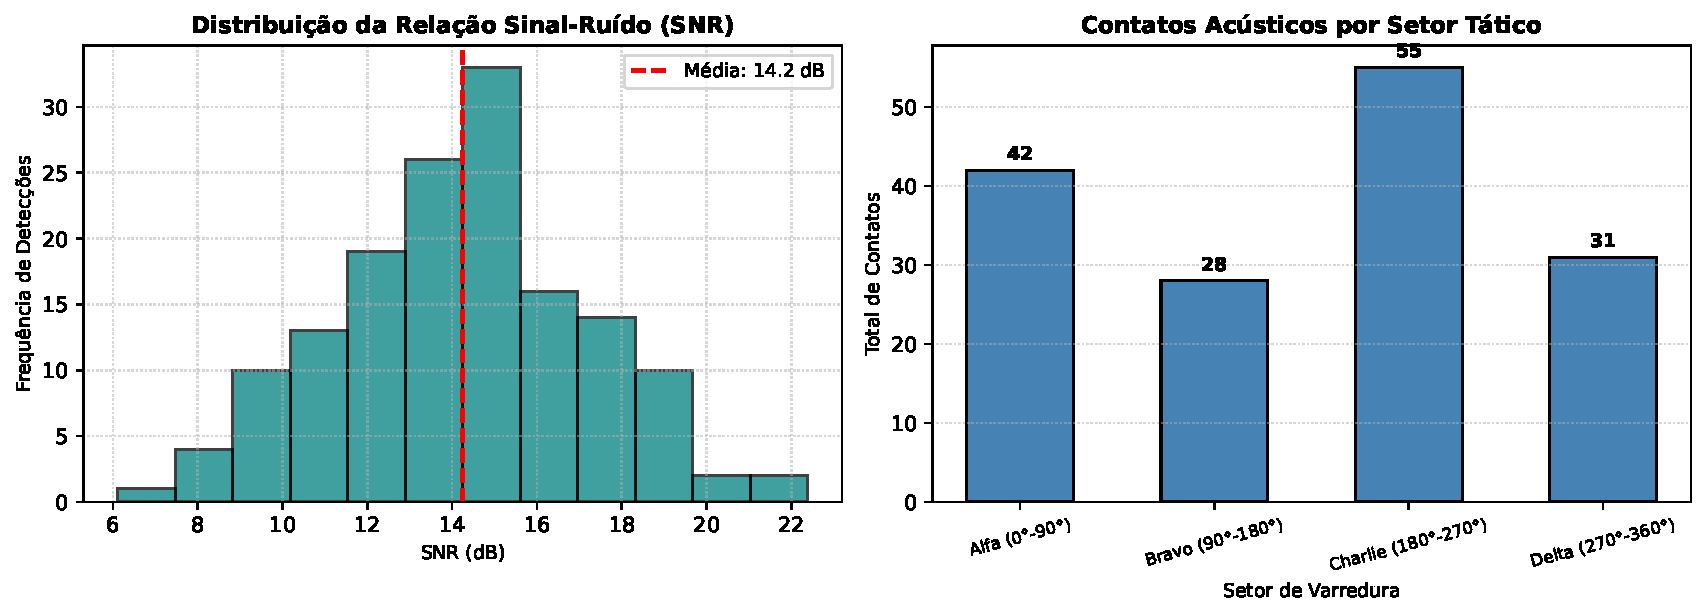
\includegraphics[width=0.98\linewidth]{body/Lista_12/figures/fig_Q10.pdf}
    \captionof{figure}{Dashboard acústico gerado: histograma de SNR com média vertical e gráfico de barras com contatos por setor.}
\end{center}
\fi
